\chapter{QR-Zerlegung}

\section{Definition}
Eine Matrix $A \in \mathbb{R}^{m \times n}$ , $m \ge n$ besitzt eine eindeutige QR-Zerlegung.
\begin{align}
	A = QR
\end{align}
mit einer orthogonalen Matrix $ Q \in \mathbb{R}^{m \times m} $ und einer oberen Dreiecksmatrix $ R \in \mathbb{R}^{n \times n}$ \cite{num1}

Eine QR Zerlegung kann mit einer Householder-Transformation berechnet werden.

\subsection{Beispiel}
Lösung eines Minimierungsproblem
\begin{align}
	\min_{x \in \mathbb{R}^n} \|Ax-b\|^2 \label{eq1}
\end{align}
mit Matrix $A \in \mathbb{R}^{m\times n}$ mit $rang(A) = n < m$ für die eine QR Zerlegung existiert.
$R$ besitzt die Gestalt 
\begin{align*}
	R=	
	\left(\begin{array}{ccc}
		*&*&* \\ 
		&*&* \\ 
		& &* \\ \hline
		& 0 &
	\end{array} \right)
	=
	\left(\begin{array}{c}
	 \\ 
	\hat{R} \\ 
	 \\ \hline
	0
	\end{array} \right) 
\end{align*}

$\hat{R}$ stellt eine obere Dreiecksmatrix dar.
Damit kann man das Minimierungs Problem wie folgt modifizieren mit $A=QR$
\begin{align}
		\min_{x \in \mathbb{R}^n} \|Ax-b\|^2 =
		\min_{x \in \mathbb{R}^n} \|Q^T(Ax-b)\|^2 =
		\min_{x \in \mathbb{R}^n} \|Rx-Q^Tb\|^2
\end{align}
Also löst
\begin{align}
Rx=Q^Tb \label{solvminqr}
\end{align}
das Minimierungsproblem (\ref{eq1}). Da $R$ eine Dreiecksmatrix ist, lässt sich (\ref{solvminqr}) leicht mit Rückwärtseinsetzen  lösen.

\section{Householder-Transformation}
Sei  $v \in \mathbb{R}^n$ ein Vektor dann wird die $n \times n$ Matrix 
\begin{align}
	H = I - 2 \dfrac{vv^T}{v^Tv}
\end{align}
als Householder-Transformation und der Vektor $v$ als Householder-Vektor bezeichnet.
Eine Householder-Transformation $H = I - 2 \dfrac{vv^T}{v^Tv}$ ist orthogonal und symmetrisch. \cite{num1}\\
Die Householder-Transformation spiegelt den Vektor $x$ auf die Achse $x_1$.
Dazu multipliziert man $H$ von links auf $x$
\begin{align}
	Hx=\alpha e_1 \label{spiegelung}
\end{align}
mit dem Skalar $\alpha \in \mathbb{R}$ und $e_1$ als ersten kanonischen Einheitsvektor. Der Householder-Vektor steht senkrecht auf der Ebene an welcher $x$ gespiegelt wird.\\
Die Abbildung \ref{fig:HHolder} veranschaulicht die Spiegelung des Vektors $x$ an der gestrichelt eingezeichneten Ebene auf die Achse $x_1$.
[Abbildung \ref{fig:HHolder}]
\begin{figure}[H]
	\centering
	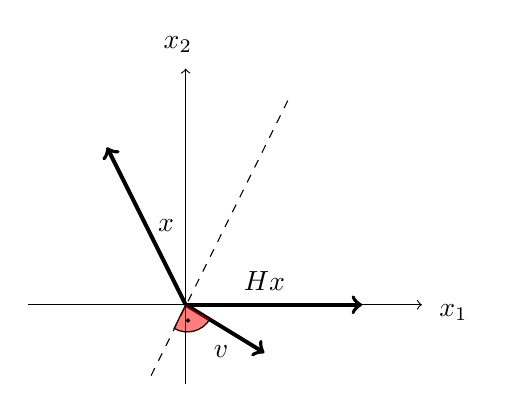
\begin{tikzpicture}

\draw[->] (-2,0) -- (3,0);
\draw[->] (0,-1) -- (0,3);

\draw[->,line width=0.5mm] (0,0) -- (-1,2);
\draw[->,line width=0.5mm] (0,0) -- (2.24,0);

\draw[dashed] (-0.44,-0.9) -- (1.34,2.68);
%\draw[->,line width=0.5mm] (0,0) -- (-0.9, 0.44);
%\draw[->,line width=0.5mm] (0,0) -- (-1,0.61);
\draw[->,line width=0.5mm] (0,0) -- (1,-0.61);





\filldraw[red, opacity=0.5] (0,0)--(-0.1467,-0.3000) arc (240:330:.3339) -- (0,0) ;
\draw[black, opacity=1] (0,0)--(-0.1467,-0.3000) arc (240:330:.3339) -- (0,0) ;
\filldraw(0.03,-0.2) circle (.02cm) ;

%Beschriftung
\draw (3.4,-0.1) node {$x_1$};
\draw (-0.1,3.3) node {$x_2$};

\draw (.45, -.6) node {$v$};
\draw (-.25, 1) node {$x$};
\draw (1,0.3) node {$Hx$};


\end{tikzpicture}
	\caption{Beispiel Householder-Transformation mit $x=(-1,2)^T$}
	\label{fig:HHolder}
\end{figure}

Householder-Transformationen können die eine Matrix $A$ wie folgt transformieren.
\begin{align*}
	H_1 A= \left( 
	\begin{array}{cccc}
	* & * & * & * \\ 
	0 & * & * & * \\ 
	0 & * & * & * \\ 
	0 & * & * & *
	\end{array}
	\right)
	\quad , \quad
	H_2 H_1 A= \left( 
	\begin{array}{cccc}
	* & * & * & * \\ 
	0 & * & * & * \\ 
	0 & 0 & * & * \\ 
	0 & 0 & * & *
	\end{array}
	\right)
\end{align*} 
So erhält man folgende Faktorisierung
\begin{align*}
	R = H_{n-1} H_{n-2}\cdot ...\cdot H_1 A \Leftrightarrow A = (H_1\cdot ...\cdot H_{n-1})R \Rightarrow Q = H_1\cdot ... \cdot H_{n-1}
\end{align*}
$Q$ ist das Produkt aller Householder-Transformationen.


\subsection{Householder Vector}
%Wie muss der Vektor $v$ aussehen damit (\ref{spiegelung}) gilt?\\
Damit (\ref{spiegelung}) gilt, muss der Vektor folgendermaßen berechnet werden. \\
Mit $Hx = x - 2\dfrac{vv^T}{v^Tv} x = x - \lambda v \overset{!}{=} \alpha e_1$ folgt $v \in \text{span}\{x - \alpha e_1\}$. \cite{num1}\\
Die Definition des Vektors $v = t(x - \alpha e_1)$ wird in $Hx = \alpha e_1 $ eingesetzt
\begin{align*}
	Hx =& x - \dfrac{2}{v^Tv}v(v^Tx) = x - 2\dfrac{v^Tx}{v^Tv}v\\
	=& x - 2\dfrac{ t(x - \alpha e_1)^Tx}{ t(x - \alpha e_1)^T t(x - \alpha e_1)} t(x - \alpha e_1)
	= x - 2\dfrac{ (x - \alpha e_1)^Tx}{ (x - \alpha e_1)^T (x - \alpha e_1)} (x - \alpha e_1)
	\\
	=& x - \dfrac{(x - \alpha e_1)^Tx}{\|x - \alpha e_1\|_2^2} (x - \alpha e_1)
	=\underbrace{\left(1 - \dfrac{2(x - \alpha e_1)^Tx}{\|x - \alpha e_1\|_2^2}\right)}_{ \overset{!}{=} 0 } x + \alpha e_1 \underbrace{\dfrac{2(x - \alpha e_1)^Tx}{\|x - \alpha e_1\|_2^2} }_{\overset{!}{=} 1} \overset{!}{=} \alpha e_1
\end{align*}

%Damit das Ergebnis $ = \alpha e_1$ erhalten wird, muss gelten
Damit das Letzte	 $=$ gilt muss 
\begin{align*}
	1 &= \dfrac{2(x - \alpha e_1)^Tx}{\|x - \alpha e_1\|^2}\\
	\Leftrightarrow (x - \alpha e_1)^T(x - \alpha e_1) &= 2 x^T x - 2\alpha x_1 \\
	\Leftrightarrow x^Tx -2\alpha x_1 + \alpha^2 &= 2 x^T x - 2\alpha x_1\\
	\Leftrightarrow \alpha &= \pm \sqrt{x^Tx}
\end{align*}

Das Vorzeichen von  $\alpha = \pm \sqrt{x^Tx}$ kann man frei wählen, um $ v = x - \alpha e_1$ zu berechnen.


%Wie ist das Vorzeichen von $\alpha = \pm \sqrt{x^Tx}$ zu wählen um $ v = x - \alpha e_1$ zu berechnen?

Wählt man das Vorzeichen positiv kann Auslöschung auftreten, falls $x$ annähernd ein positives Vielfaches von $e_1$ ist.

LAPACK \cite{DGEQR2} vermeidet die Auslöschung indem das Vorzeichen entgegengesetzt gewählt wird. Das bedeutet $x$ wird immer auf die gegenüberliegende Seite gespiegelt.

Im Skript von Numerik 1 \cite{num1} wird das Vorzeichen immer positiv gewählt\\ $\alpha = |\sqrt{x^Tx}| = \|x\|_2$. Eine mögliche Auslöschung im Fall $ x_1 > 0$ wird hier durch die folgende Umformung vermieden.
\begin{align*}
	v_1 = x_1 - \|x\|_2 = \dfrac{x_1^2 - \|x\|_2^2}{x_1 + \|x\|_2}
	=\dfrac{-(x_2^2+...+x_n^2)}{x_1 + \|x\|_2}
\end{align*}


%Der Vorteil bei der von LAPACK verwendeten Methode ist, dass hier nur die Norm berechnet werden muss, wohingegen bei dem anderen Algorithmus das Skalarprodukt $x^Tx$ berechnet werden muss. Dies kann bei Vektoren mit vielen Einträgen und großen Werten zu einem Überlauf führen. Es muss jedoch ein Algorithmus gewählt werden, der die Norm berechnet $\|x\|=\sqrt{x^Tx}$ ohne das Skalarprodukt explizit auszurechnen.

Um den Vektor $v$ später auf der frei werdenden Diagonalen von $A$ speichern zu können wird er auf $v_1 = 1$ normiert. Dies geschieht mit 
\begin{align}
	v = \dfrac{x - \alpha e_1}{x_1 - \alpha}
	\label{eq:calcV}
\end{align}

Mit der Normierung kann man den Faktor $\tau = \dfrac{2}{v^Tv}$ berechnen. Setze dazu (\ref{eq:calcV}) in die Definition von $\tau$ ein.
\begin{align*}
	\tau = \dfrac{2}{v^Tv} = \dfrac{2 (x_1 - \alpha)^2}{(x - \alpha e_1)^T (x - \alpha e_1)} = \dfrac{2 (x_1 - \alpha)^2}{\|x\|^2_2 - 2\alpha x^Te_1 + \alpha^2} =  \dfrac{2 (x_1 - \alpha)^2}{ 2\alpha (\alpha - x_1)} = \dfrac{x_1 - \alpha}{\alpha}
\end{align*}

Mit dem Faktor $\tau = \dfrac{2}{v^Tv}$ kann man die Householder-Transformation schreiben als
\begin{align*}
	H = I - 2 \dfrac{vv^T}{v^Tv} = I - \tau v v^T
\end{align*}

%Das macht man, weil die Berechnung des Skalarprodukts relativ aufwändig ist. Da man das Skalarprodukt zur Berechnung des Householder-Vektors benötigt, kann man damit direkt den Faktor $\tau$ berechnen.


\begin{algorithm}
	\caption{Housholder-Vector(LAPACK DLARFG)}
	\begin{algorithmic}
		\State Input: $x \in \mathbb{R}^n$ 
		\State $\alpha = -1 * \text{sign}(x_1) \|x\|_2$
		\State $\tau = \dfrac{x_1 - \alpha}{\alpha}$
		\State $v=\dfrac{x - \alpha e_1}{x_1 - \alpha}$
		\State Output: Householder-Vektor $v$, $\tau$
	\end{algorithmic} 
	\label{alg:unblockedqr}
\end{algorithm}


\subsection{Householder-Transformation anwenden}
Ein aufwändiges Matrix-Matrix-Produkt kann bei der Anwendung einer Housholder-Transformation $H = I - \tau vv^T$ auf die Matrix $A$ umgangen werden, indem man geschickt klammert.
\begin{align*} 
H A =(I - \tau vv^T) A= A - \tau (vv^T )A = A - \tau v(v^TA)
\end{align*}
Statt eines Matrix-Matrix-Produkts muss man nur ein Matrix-Vektor-Produkt und ein dyadisches Produkt berechnen.
%Das Matrix-Vektor-Produkt und das dyadische Produkt haben nur einen Aufwand von $O(n^2)$.

Das führt zum Algorithmus \ref{alg:unblockedqr}. 
\begin{algorithm}
	\caption{Ungeblockte Housholder-Transformation}
	\begin{algorithmic}
	\State Input: $A \in \mathbb{R}^{m \times n}$
	\For {i = 0 : n}
		\State ($v_i$, $\tau_i$) $\leftarrow$ housevector($A(i:m,i)$)
		\State $w \leftarrow v^T*A(i:m,i:n)$ (dgemv)
		\State $ A(i:m,i:n) \leftarrow \tau * v * w + A $ (dger)
		\If {i > m}
			\State $A(i + 1 : m, i) \leftarrow v(2 : m - i + 1)$
		\EndIf
	\EndFor	
	\State Output: $A$ QR zerlegt, Vektor $\tau \in \mathbb{R}^n$
\end{algorithmic} 
\label{alg:unblockedqr}
\end{algorithm}

Matizen sind 0 indizeiert notiert

Dieser Algorithmus \ref{alg:unblockedqr} überschreibt die Matrix $A$ mit $R$.
Aufgrund der Dreiecksstruktur von $R$,
können unter der Diagonale die Housholder-Vektoren gespeichert werden. 
Die Householder-Vektoren haben die Form 
\begin{align*}
v^{(j)} = ( \underbrace{0,...,0}_{j-1},1,	v_{j+1}^{(j)},...,v_{m}^{(j)}  )
\end{align*}
Da die ersten $j-1$ Einträge Null sind und der Vektor so normiert wurde das der $j$ Eintrag gleich 1 ist, müssen die ersten $j$ Einträge nicht gespeichert werden.
Die Householder-Vektoren können somit unterhalb der Diagonalen gespeichert werden.
Die Matrix $A$ hat die Form
\begin{align*}
	A = 
	\left(\begin{array}{ccc}
	r_{1,1}   &  r_{1,2}  & r_{1,3} \\ 
	v_2^{(1)} &  r_{2,2}  & r_{2,3} \\ 
	v_3^{(1)} & v_3^{(2)} & r_{3,3} \\ 
	v_4^{(1)} & v_4^{(2)} & v_4^{(3)}
	\end{array} \right) 
\end{align*}


\section{Geblockte QR-Zerlegung}
Ein geblockter Algorithmus ist sinnvoll, um bei großen Matrizen den Cache optimal zu nutzen.

Im folgenden wird ein geblockter Algorithmus beschrieben wie er auf von LAPACK verwendet wird. Die entsprechende Funktion bei LAPACK heißt \glqq DGEQRF\grqq{} \cite{DGEQRF}.

Die Idee beim geblockten Algorithmus ist die Matrix in Blöcke aufzuteilen, die geblockte QR-Zerlegung für die Blöcke zu berechnen und die dabei verwendeten Householder-Transformationen auf den Rest der Matrix anzuwenden.


Betrachte dazu die Matrix $A \in \mathbb{R}^{m \times n}$ geblockt, mit einer geeigneten Blockgröße $bs$.
\begin{align}
	A = \left(\begin{array}{l|l}
	A_{0, 0} & A_{0, \text{bs}} \\ \hline
	A_{\text{bs}, 0}   & A_{\text{bs}, \text{bs}} 	
	\end{array} \right) \label{equ:blockA}
\end{align}
Die Abbildung \ref{fig:blockA} zeigt schematisch die Partitionierung von A.

Die Blockgröße $bs$ wird so gewählt das die Geschwindigkeit der ungeblockten QR-Zerlegung für den Block $ \left(\dfrac{A_{0, 0}}{A_{\text{bs}, 0}} \right)$ optimal ist.

Für diesen Block wird nun die  QR-Zerlegung mit dem ungeblockten Algorithmus (Algorithmus \ref{alg:unblockedqr}) berechnet.
\begin{align}
	\left(\begin{array}{l} 
	A_{0, 0} \\ \hline
	A_{\text{bs}, 0}
	\end{array}\right)
	\leftarrow
	\left(\begin{array}{l} 
	Q_{0, 0}  \backslash R_{0,0} \\ \hline
	Q_{\text{bs}, 0} 
	\end{array}\right)
\end{align}

Im Block $A_{0, 0}$ steht nun auf und über der Diagonalen $R_{0,0}$. Unterhalb der Diagonalen und im Block $A_{\text{bs}, 0}$ stehen die Householder-Vektoren.

Nun muss man die bei der ungeblocketn QR-Zerlegung verwendeten Housholder-Transformationen auf die Restliche Matrix $ \left(\dfrac{A_{0, \text{bs}}}{A_{\text{bs}, \text{bs}}} \right)$ anwenden.



Man kann das Produkt mehrerer Householder-Transformationen schreiben als
\begin{align*}
H_1H_2...H_k = I - VTV^T \qquad \text{mit}\qquad H_i = I - \tau_i v_iv_i^T
\end{align*} \cite{Joffrain:2006:AHT:1141885.1141886}

Die Anwendung der Matrix $I - V*T*V^T$ auf $\left(\dfrac{A_{\text{bs}, \text{bs}}}{A_{\text{bs}, \text{bs}}} \right)$ erfolgt in 2 Schritten.

Zuerst wird von der Funktion \glqq larft \grqq{}  die Matrix $T$ berechnet.
Dann wird $I - V*T*V^T$ von der Funktion \glqq larfb\grqq{} auf $\left(\dfrac{A_{\text{bs}, \text{bs}}}{A_{\text{bs}, \text{bs}}} \right)$ angewendet.


\begin{align}
	\left(\begin{array}{l} 
	A_{0, \text{bs}} \\ \hline
	A_{bs, \text{bs}}
	\end{array}\right)
	\leftarrow
	H^T \left(\begin{array}{l} 
	A_{0, \text{bs}} \\ \hline
	A_{bs, \text{bs}}
	\end{array}\right)
\end{align}

%Betrachte nun den Block $A_{bs, \text{bs}}$ wie in (\ref{equ:blockA}), in der Abbildung \ref{fig:blockA} gestrichelt Dargestellt.

Der Block $A_{bs, \text{bs}}$ wird erneut aufgeteilt. Das ist in Abbildung \ref{fig:blockA} gestrichelt dargestellt.

Fahre solange fort bis $A_{bs, \text{bs}}$ gleich der Blockgröße ist.
\begin{figure}[H]
	\centering
	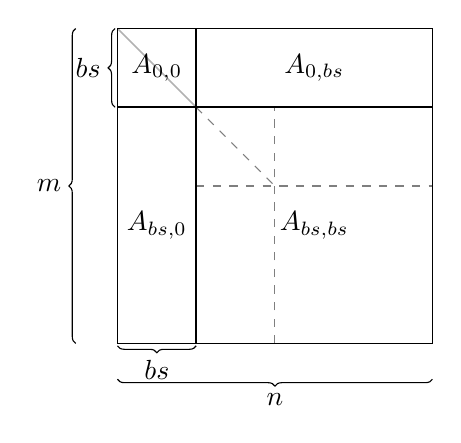
\begin{tikzpicture}
\draw[semithick] (0,0) -- (4,0) -- (4,4) -- (0,4) -- (0,0);

\draw[semithick] (1,0) -- (1,4);
\draw[semithick] (0,3) -- (4,3);
\draw[semithick,opacity=0.3] (0,4) -- (1,3);

\draw[dashed,opacity=0.5] (2,0) -- (2,3);
\draw[dashed,opacity=0.5] (1,2) -- (4,2);
\draw[dashed,opacity=0.5] (1,3) -- (2,2);


\draw (0.5,3.5) node {$A_{0,0}$};
\draw (0.5,1.5) node {$A_{bs,0}$};
\draw (2.5,3.5) node {$A_{0,bs}$};
\draw (2.5,1.5) node {$A_{bs,bs}$};
\draw[decorate, decoration={brace,mirror}, yshift=-.2ex]  (0,0) -- node[below=0.4ex] {$bs$}  (1,0);
\draw[decorate, decoration={brace}, xshift=-.2ex]  (0,3) -- node[left=0.4ex] {$bs$}  (0,4);
\draw[decorate, decoration={brace,mirror}, yshift=-3ex]  (0,0) -- node[below=0.4ex] {$n$}  (4,0);
\draw[decorate, decoration={brace}, xshift=-3.5ex]  (0,0) -- node[left=0.4ex] {$m$}  (0,4);

\end{tikzpicture}
	\caption{Partitionierung vom A}
	\label{fig:blockA}
\end{figure}

\subsection{Berechnung der Matrix $T$}
Die Funktion \glqq larft\grqq{} berechnet die Matrix $T$. 

Sie bekommt eine Dreiecksmatrix $V \in \mathbb{R}^{m \times k}$ einen Vektor $\tau \in \mathbb{R}^k$ und eine Matrix $T\in \mathbb{R}^{k\times k}$ übergeben. 

In der Dreiecksmatrix $V$ stehen die Householder-Vektoren,
im Vektor $\tau$ die zu den Householder-Vektoren gehörende $\tau_i$.

Die Funktion berechnet eine obere Dreiecksmatrix $T$ so dass
\begin{align*}
	H_1H_2...H_k = I - VTV^T \qquad \text{mit}\qquad H_i = I - \tau_i v_iv_i^T
\end{align*}

Warum und wie das Funktoniert wird hier beschreiben \cite{Joffrain:2006:AHT:1141885.1141886}.




\subsection{Anwenden von $I - VTV^T$ larfb}

Die Funktion \glqq larfb \grqq{} wendet die Matrix $I - VTV^T$ auf eine Matrix $C$ an.

Sie bekommt eine untere Dreiecksmatrix $V \in \mathbb{R}^{m \times k}$, eine obere Dreiecksmatrix $T \in \mathbb{R}^{k \times k}$ und eine Matrix $C \in \mathbb{R}^{m \times n }$ übergeben.

In der Dreiecksmatrix $V$ stehen die Householder-Vektoren,
im Vektor $\tau$ die zu den Householder-Vektoren gehörende $\tau_i$.
Die Matrix $C$ wird upgedatet indem die  Block Reflector Matrix $ 	H = C - V T V^T $ von rechts auf die Matrix $ C $ angewendet wird. 

Ein weiterer Übergabeparameter gibt an ob die Block Reflector Matrix transponiert werden soll.
Die Funktion berechnet also
\begin{align*}
	C \leftarrow H C = C - V T V^T C \quad \text{oder} \quad 	C \leftarrow H^T C = C - V T^T V^T C
\end{align*}

Der Zweck der Funktion ist es die Householder-Transformationen, die bei der Bereicherung der QR-Zerlegung für einen Block entstanden sind, auf die restliche Matrix anzuwenden.
Die Abbildung \ref{fig:patrA} zeigt wie die Matrix $A$ für die Funktion Partitioniert wird.
\begin{figure} [H]
	\centering
	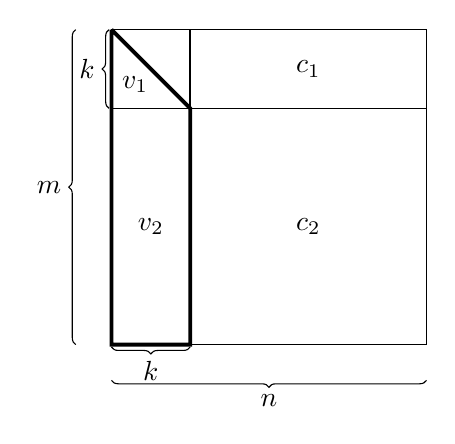
\begin{tikzpicture}
\draw[semithick] (0,0) -- (4,0) -- (4,4)-- (0,4)-- (0,0);


\draw[semithick] (1,0) -- (1,4);
\draw[semithick] (0,3) -- (4,3);
\draw[line width=0.5mm] (0,4) -- (0,0) -- (1,0) -- (1,3) -- (0,4);


\draw[decorate, decoration={brace,mirror}, yshift=-.2ex]  (0,0) -- node[below=0.4ex] {$k$}  (1,0);
\draw[decorate, decoration={brace}, xshift=-.2ex]  (0,3) -- node[left=0.4ex] {$k$}  (0,4);
\draw[decorate, decoration={brace,mirror}, yshift=-3ex]  (0,0) -- node[below=0.4ex] {$n$}  (4,0);
\draw[decorate, decoration={brace}, xshift=-3ex]  (0,0) -- node[left=0.4ex] {$m$}  (0,4);

\draw (0.3,3.3) node {$v_1$};
\draw (0.5,1.5) node {$v_2$};
\draw (2.5,3.5) node {$c_1$};
\draw (2.5,1.5) node {$c_2$};



\end{tikzpicture}
	\caption{Partitionierung vom A für larfb}
	\label{fig:patrA}
\end{figure}
Falls $m > k $ werden die Matrizen $V$ und $C$ aufgeteilt in $V=\left(\dfrac{V_1}{V_2}\right)$ und $C=\left(\dfrac{C_1}{C_2}\right)$.
%Sodass $V_1 \in \mathbb{R}^{k \times k}$ und $C \in \mathbb{R}^{k \times n}$
Dabei wird $V$ genau so geteilt, dass $V_1 \in \mathbb{R}^{k\times k}$ der quadratisch Dreiecksteil der Matrix ist und $V_2 \in \mathbb{R}^{m-k\times k}$ der Rest der Matrix. Die Matrix $C$ wird in $C_1 \in \mathbb{R}^{k \times n}$ und $C_2 \in \mathbb{R}^{m-k \times n}$  aufgeteilt. Die Aufteilung ist so gewählt das das Matrix-Matrix-Produkt $V_1 \cdot C_1$ und $V_2 \cdot C_2$ möglich ist.\\
Diese Aufteilung ist notwendig da die BLAS-Funktion trmm (matrix-matrix product where one input matrix is triangular) nur für Quadratische Dreiecksmatrizen implementiert ist.

Im Fall $ m = k $ ist die Aufteilung nicht notwendig da $ V $ quadratisch ist.




\begin{align*}
	C \leftarrow  C - \underbrace{V T V^T C}\\
	V \cdot T \cdot V^T \cdot C\\ 
	(C^T \cdot V \cdot T^T \cdot V^T)^T 
\end{align*}



Dies führt zu den
\begin{algorithm}[H]
	\caption{Block reflector anwenden}
	\label{alg:applyblockref}
	\begin{algorithmic}
		\State 	$W \leftarrow C_1^T$ (copy)
		\State	$W \leftarrow W * V_1 $ (trmm)
		\If {m > k}
			\State $W \leftarrow W + C_2^T*V_2$ (gemm)
		\EndIf
		\State 	$ W \leftarrow W * T^T \quad \text{or}\quad  W * T$ (trmm)
		\If {m > k}
			\State $C_2 \leftarrow C_2 - V_2 * W^T$ (gemm)
		\EndIf
		\State 	$ W \leftarrow W * V_1^T $ (trmm)
		\State 	$ C_1 \leftarrow C_1 - W^T $
	\end{algorithmic}
\end{algorithm}





\subsection{Iterativer Algorithmus}
\begin{algorithm}[H]
	\caption{Iterativer Algorithmus}
	\label{alg::italg}
	\begin{algorithmic}
		\For {i = 0 : n}
			\State QR = A;
			\If {i + ib > n}
				\State Calc T: $H=I-VTV^T$
				\State Apply H: $A=H^TA$
			\EndIf
		\EndFor
	\end{algorithmic}
\end{algorithm}
